\documentclass [a4paper] {report}
\usepackage{amsmath,amssymb,amsthm, bbm, graphicx,listings,braket,subfig,titlesec,cleveref,lipsum,mcode,xcolor-patch, textcomp,float,booktabs,siunitx, listings}
\usepackage[authoryear]{natbib}
\usepackage[section]{placeins}
\usepackage[margin=2.2cm]{geometry}
\titleformat{\chapter}{\normalfont\huge}{\thechapter.}{20pt}{\huge \bf}

\DeclareMathOperator*{\argmin}{arg\,min}
\DeclareMathOperator*{\argmax}{arg\,max}
\newcommand{\norm}[1]{\left\lVert #1 \right\rVert}

\begin{document}
	
	\begin{titlepage}
		\begin{center}
			
			\textsc{\LARGE IN4320 Machine Learning}\\[1.25cm]
			
			\rule{\linewidth}{0.5mm}\\[1.0cm]
			{\huge \bfseries Exercises: Reinforcement Learning }\\[0.6cm]
			\rule{\linewidth}{0.5mm}\\[1.5cm]
			
			\begin{minipage}{0.4\textwidth}
				\begin{flushleft} \large	
					\emph{Author:}\\
					\textsc{Milan Niestijl, 4311728}
				\end{flushleft}
			\end{minipage}
			
			\vfill
			{\large \today}
		\end{center}
	\end{titlepage}
	
	\section*{Exercise 1}
	\textbf{Claim}\\
	The return $R_{t} = \sum_{h=0}^{\infty}\gamma^{h}r_{t+h+1}$ is bounded for $0\leq \gamma<1$ and bounded rewards $-10\leq r_{t+h+1}\leq 10$ for all $h\in \mathbb{N}$.\\\\
	\textbf{Proof}\\
	Using the geometric series, we find:
	$$|R_{t}| \leq \sum_{h=0}^{\infty}|\gamma^{h}r_{t+h+1}| \leq \sum_{h=0}^{\infty}10 \gamma^{h} = {10 \over 1-\gamma} < \infty$$
	
	\section*{Exercise 2}
	The Q-function is shown after each iteration in the tables \ref{Qtable}.
	
	\begin{table}[H]
		\centering
		\caption{Q-value for different iterations.}
		\label{Qtable}
		\begin{tabular}{ll|llllll}
			& Action\textbackslash State    & 1 & 2 & 3 & 4 & 5 & 6 \\ \cmidrule{2-8}
	$i=0:$	& Left 				& 0 & 0 & 0 & 0 & 0 & 0 \\ 
			& Right 			& 0 & 0 & 0 & 0 & 0 & 0 \\ \cmidrule{2-8}
	$i=1:$	& Left 				& 0 & 1 & 0 & 0 & 0 & 0 \\ 
			& Right 			& 0 & 0 & 0 & 0 & 5 & 0 \\ \cmidrule{2-8}
	$i=2:$	& Left 				& 0 & 1 & 0.5 & 0 & 0 & 0 \\ 
			& Right 			& 0 & 0 & 0 & 2.5 & 5 & 0 \\ \cmidrule{2-8}
	$i=3:$	& Left 				& 0 & 1 & 0.5 & 0.625 & 1.25 & 0 \\ 
			& Right 			& 0 & 0.625 & 1.25 & 2.5 & 5 & 0 \\ 
		\end{tabular}		
	\end{table}
	
	\noindent
	The resulting optimal policy is shown in table \ref{optPolicy}.
	
	\begin{table}[H]
		\centering
		\caption{Optimal policy for $\gamma=0.5$.}
		\label{optPolicy}
		\begin{tabular}{l|llllll}
			$s$    			& 1 & 2 & 3 & 4 & 5 & 6 \\ \hline
			$\pi(s)$			& Right & Left & Right & Right & Right & Right \\ 
		\end{tabular}
	\end{table}
	
	
	\section*{Exercise 3}
	The optimal value functions for $\gamma \in \{ 0,0.1, 0.9, 1 \}$ are shown in table \ref{optQs}.
	Note that $\gamma=1$ will work here because the reward function has a finite horizon.
	
	\begin{table}[H]
		\centering
		\caption{$Q*$ for various values of the discount factor $\gamma$.}
		\label{optQs}
		\begin{tabular}{ll|llllll}
						&  Action\textbackslash State    & 1 & 2 & 3 & 4 & 5 & 6 \\ \cmidrule{2-8}
	$\gamma=0.0:$		& Left 				& 0 & 1 & 0 & 0 & 0 & 0 \\ 
						& Right 			& 0 & 0 & 0 & 0 & 5 & 0 \\ \cmidrule{2-8}
	$\gamma=0.1:$		& Left 				& 0 & 1 & 0.1 & 0.01 & 0.005 & 0 \\ 
						& Right 			& 0 & 0.01 & 0.05 & 0.5 & 5 & 0 \\ \cmidrule{2-8}
	$\gamma=0.9:$		& Left 				& 0 & 1 & 3.2805 & 3.645 & 4.05 & 0 \\ 
						& Right 			& 0 & 3.645 & 4.05 & 4.5 & 5 & 0 \\ \cmidrule{2-8}
	$\gamma=1:$			& Left 				& 0 & 1 & 5 & 5 & 5 & 5 \\ 
						& Right 			& 0 & 5 & 5 & 5 & 5 & 0 \\ 
		\end{tabular}
	\end{table}

	\section*{Exercise 4}
	In figure \ref{QErrors}, the 2-norm error of the learned Q-function is plotted versus the number of iterations for several values of the exploration rate $\epsilon$ and the learning rate $\alpha$. It can be seen that for larger values of $\epsilon$, the error decreases faster. This is explained by the fact that more often a random action is taken, which effectively allows the system to gain more new information and alter its values accordingly. Similarly, for larger values of $\alpha$, the learned Q-function on average updates with larger steps, which is reflected in the figure by the fact that the error makes larger 'jumps'. In this case, this causes the algorithm to converge faster.
	
	\begin{figure}[H]
		\begin{center}
			\includegraphics[scale=0.5]{Images/QErrors.png}
			\caption{2-Norm errors of the obtained Q-values for different values of $\epsilon$ and $\alpha$ versus the number of iterations performed. Ten realisations are shown in each case.}
			\label{QErrors}
		\end{center}
	\end{figure}
	
	\section*{Exercise 5}
	In this case, q-iteration still converges as it uses the transition probabilities. The iterations are thus deterministic. Q-learning however, no longer converges as the iterations are stochastic in nature. The values keep changing depending on whether the robot fails or not during that step, never allowing the algorithm to converge. In figure 2, the 2-norm errors of the obtained Q-values are shown, where the result of q-iteration is taken to be the 'true' value. It can be seen that for smaller values of the learning rate $\alpha$, the resulting standard deviation becomes smaller.
	
	\begin{figure}[H]
		\begin{center}
			\includegraphics[scale=0.35]{Images/QErrors_0_2.png}
		\end{center}
		\begin{center}
			\includegraphics[scale=0.35]{Images/QErrors_0_05.png}
		\end{center}
		\begin{center}
			\includegraphics[scale=0.35]{Images/QErrors_0_01.png}
		\end{center}
		\label{QErrors2}
		\caption{2-Norm errors of the obtained Q-values for different values of $\alpha$ versus the number of iterations performed. Ten realisations are shown in each case.}
	\end{figure}
	
	\newpage
	\section*{Exercise 5}
	Next, we implement value function approximation with radial basis functions for Q-learning. Pseudo-code is shown below.
	
	\begin{lstlisting}
	Algorithm: Q-Learning
	Inputs: MDP, eps, alpha, activationFunctions
	
	Initialize weights with zeros.
	Loop:
		s <- get random state
		a <- argmax Q(s,a)
		With probability eps:
			a <- get random action
		snew, reward <- make transition(s,a)
		TD <- reward + discount*(max Q(snew,a)) - Q(s,a)
		W[a] <- W[a] + alpha*TD*evalActFuncs(s)
		
	where
		def evalActFuncs(s):
			evaluated  <- [ f(s) for f in activationFunctions ]
			normalized <- evaluated/sum(evaluated)
			return normalized
	
		def Q(s,a):
			return dotProduct(W[a],evalActFuncs(s)) 	
	\end{lstlisting}
	
	\noindent
	The result is tested on the scenario described in the assignment. It is expected that for a larger number of functions, the approximation becomes more accurate. To start off, the result is tested using six radial basis functions with the same variance $c^{2}$, located at the six different states. Parameters $\epsilon=0.4$ and $\alpha=0.3$ are used. To verify that the method works, it is first tried in the simpler case of $\sigma^{2}=0$. The resulting approximation of the Q-function is shown in figure \ref{Qfunc1}
	
	\begin{figure}[H]
		\begin{center}
			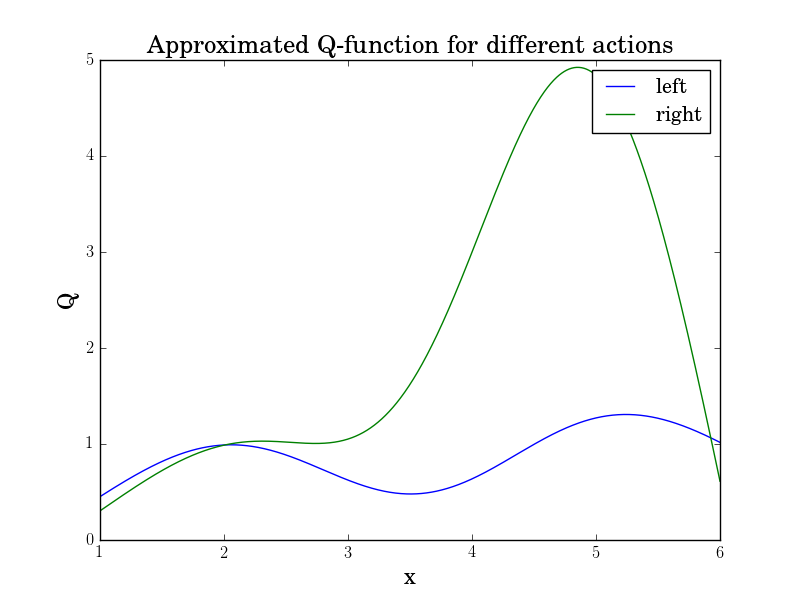
\includegraphics[scale=0.4]{Images/q_approx6.png}
			\caption{Approximation of the Q-function using six radial basis functions with variance $c=1$ located at the six different states.}
			\label{Qfunc1}
		\end{center}
	\end{figure}
	
	\noindent
	Next, we set $\sigma^{2}=0.01$ and try the algorithm using 100 activation functions, evenly spaced with width $c={100 \over 6}$.  The result is shown in figure \ref{Qfunc2}. Comparing this result with table \ref{Qtable}, it can be seen that the Q-functions match, verifying that the algorithm is converging towards the right solution. However, as the Q-function has discontinuities, a Gibbs phenomenon can be observed.
	
	\begin{figure}[H]
		\begin{center}
			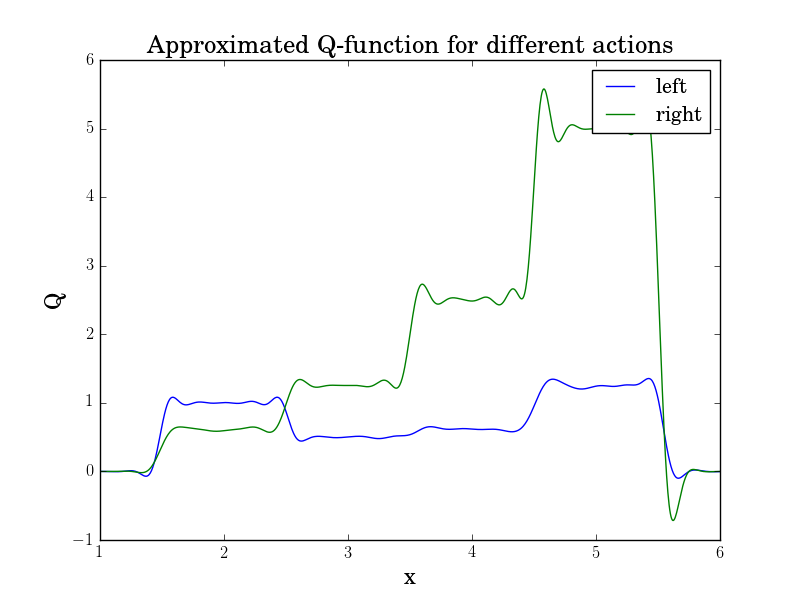
\includegraphics[scale=0.4]{Images/q_approx100.png}
			\caption{Approximation of the Q-function using 100 radial basis functions with variance $c={100 \over 6}$ located at the six different states.}
			\label{Qfunc2}
		\end{center}
	\end{figure}
	
	\noindent
	Next, we are interested in the speed of convergence. However, unlike in the discrete case, we can no longer compare to the result of q-iteration. Instead, we look at the expected maximum reward $R$. Let $s_{0}$ be the initial position of the robot. The expected reward  $R$ is then defined by $\mathbb{E}(Q^{*}(s_{0}))$. If we assume all positions are equally likely, then $s_{0}$ is a uniformly distributed random variable and this expression becomes:
	$$ R = {1\over 5} \int_{1}^{6} Q^{*}(s) ds$$
	Which can now be approximated by numerical integration. The trapezoidal rule was used to approximate the integral. In figure \ref{reward}, the expected maximal reward $R$ is plotted versus the number of iterations. It can be seen that $R$ does indeed converge, but the algorithm converges much slower as in the discrete case, shown in \ref{QErrors}. \\
	Note that if in the discrete case the probability of starting in one of the absorbing states 1 and 6 is half that of the others (which is the discrete analogue of the statement that a terminal state is reached when $s<1.5$ or $s>5.5$), then the expected maximal return $R_{d}$ is given by:
	$$ R_{d} = {1\over 5}\left( 1+1.25+2.5+5.0 \right)=1.95 $$
	Which is also the value $R$ converges towards.
	
	\begin{figure}[H]
		\begin{center}
			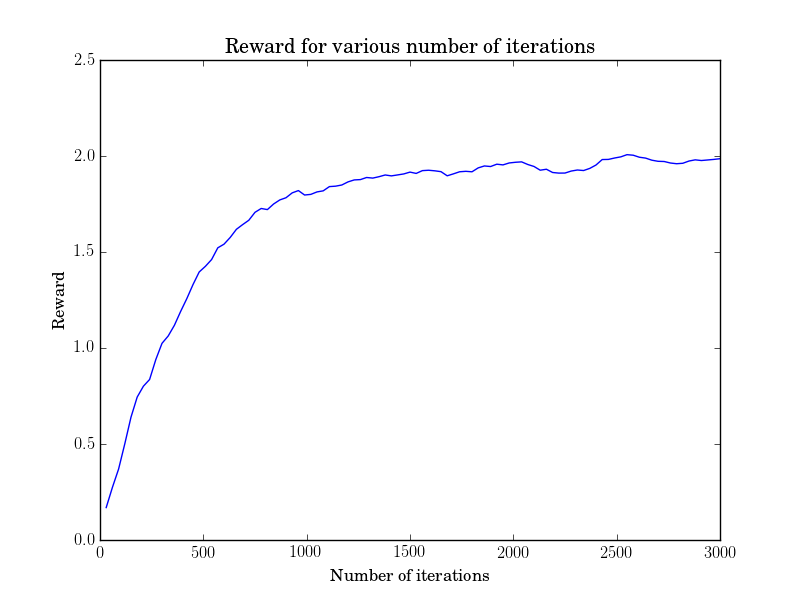
\includegraphics[scale=0.4]{Images/expected_return01.png}
			\caption{Expected maximal reward versus the number of iterations.}
			\label{reward}
		\end{center}
	\end{figure}
	
	\newpage
	\section*{Exercise 7}
	Lastly, we implement SARSA in with an RBF-network, approximating the state-action value function. Pseudo code is shown below. The main difference is the update rule of the weights. Q-Learning uses the optimal policy to evaluate Q-values, which differs from the policy that is learning (which uses an exploration/exploitation trade-off). It is therefore an off-policy algorithm. SARSA on the other hand is on-policy; it follows the epsilon-greedy policy that is learning to determine the new action and uses its corresponding Q-value to update the weights, which may not be the optimal one. SARSA may be more appropriate in situations where taking a random action may have disastrous effects in certain states, as the Q-values corresponding to these actions are down valued accordingly.
	
	\begin{lstlisting}
	Algorithm: SARSA
	Inputs: MDP, eps, alpha, activationFunctions
	
	Initialize weights with zeros.
	Loop:
		s <- get random state
		a <- argmax Q(s,a')
		With probability eps:
			a <- get random action
		snew, reward <- make transition(s,a)
		anew = argmax(Q,snew,a')
		With probability eps:
			anew = get random action
		TD <- reward + discount*Q(snew,anew) - Q(s,a)
		W[a] <- W[a] + alpha*TD*evalActFuncs(s)
	
	where
		def evalActFuncs(s):
			evaluated  <- [ f(s) for f in activationFunctions ]
			normalized <- evaluated/sum(evaluated)
			return normalized
		
		def Q(s,a):
			return dotProduct(W[a],evalActFuncs(s)) 	
	\end{lstlisting}
		
	Using $\alpha=0.4$, $\gamma=0.5$ and 100 RBF functions, the approximated Q-function is shown in figure \ref{SARSA_Qfunc}. It can be seen that the algorithm does indeed converge to right Q-function. Next, the expected maximal reward $R$ is shown for various values of $\epsilon$ in figure \ref{SARSA_reward}. It is observed that for larger values of $\epsilon$, $R$ converges to a lower value, which is caused by a random action yielding a suboptimal Q-value more often. 

	\begin{figure}[H]
		\begin{center}
			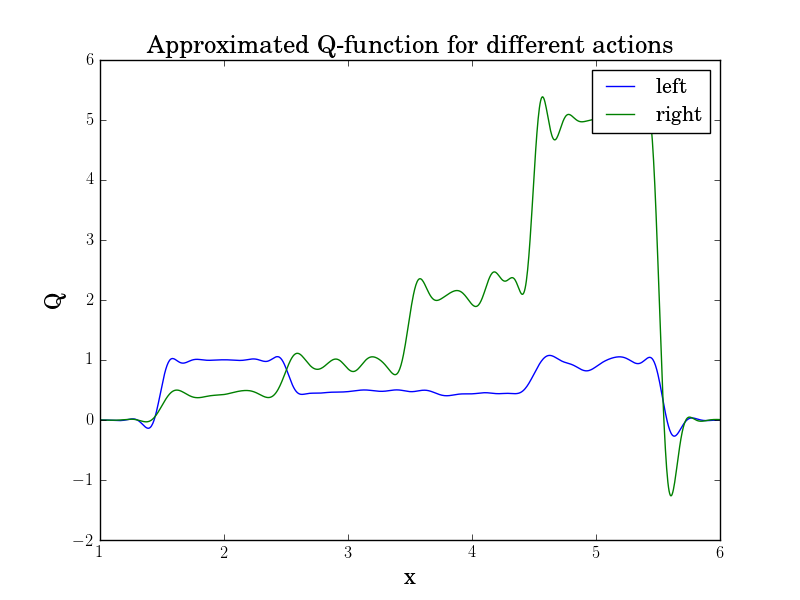
\includegraphics[scale=0.4]{Images/SARSA_Q_Approx.png}
			\caption{Approximated Q-function using the SARSA algorithm.}
			\label{SARSA_Qfunc}
		\end{center}
	\end{figure}
		
	\begin{figure}[H]
		\begin{center}
			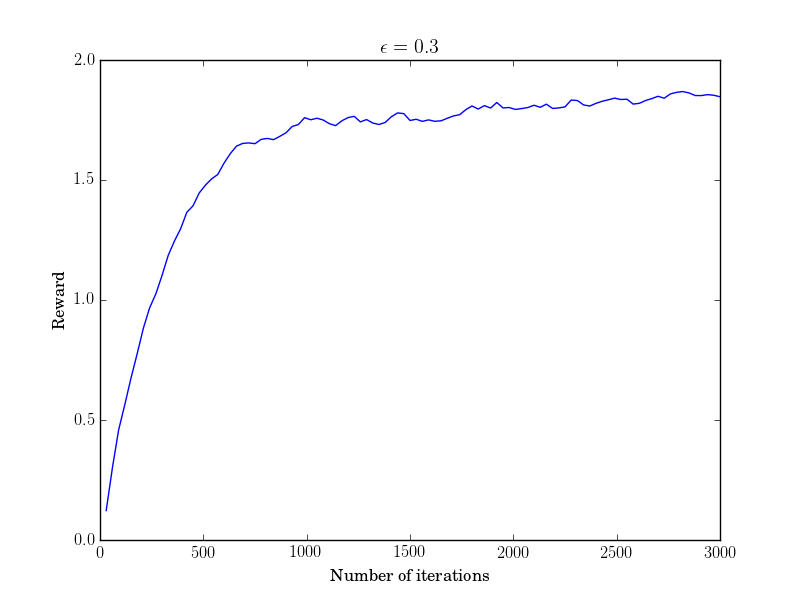
\includegraphics[scale=0.4]{Images/return_SARSA_eps_0_3.png}
			\caption{Expected maximal reward versus the number of iterations.}
		\end{center}
		
		\begin{center}
			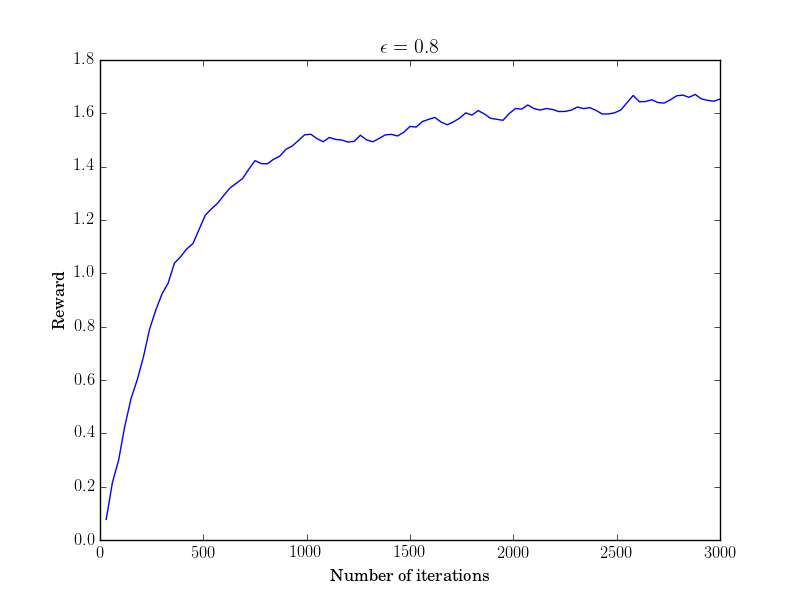
\includegraphics[scale=0.4]{Images/return_SARSA_eps_0_8.png}
			
		\end{center}
		\caption{Expected maximal reward versus the number of iterations for different values of $\epsilon$.}
		\label{SARSA_reward}
	\end{figure}

\end{document}